\documentclass[type=bachelor, fontset=custom]{thuthesis}
% 选项:
%   type=[bachelor|master|doctor|postdoctor], % 必选
%   secret,                                   % 可选
%   pifootnote,                               % 可选(建议打开)
%   openany|openright,                        % 可选,基本不用
%   arial,                                    % 可选,基本不用
%   arialtoc,                                 % 可选,基本不用
%   arialtitle                                % 可选,基本不用

% 所有其它可能用到的包都统一放到这里了,可以根据自己的实际添加或者删除。
\usepackage{thuthesis}

% 自定义包和命令
\usepackage{custom}

% 定义所有的图片文件在 figures 子目录下
\graphicspath{{figures/}}

% 可以在这里修改配置文件中的定义。导言区可以使用中文。
% \def\myname{薛瑞尼}

\begin{document}

%%% 封面部分
\frontmatter
\thusetup{
  %******************************
  % 注意:
  %   1. 配置里面不要出现空行
  %   2. 不需要的配置信息可以删除
  %******************************
  %
  %=====
  % 秘级
  %=====
  secretlevel={秘密},
  secretyear={10},
  %
  %=========
  % 中文信息
  %=========
  ctitle={清华大学学位论文 \LaTeX\ 模板\\使用示例文档 v\version},
  cdegree={工学硕士},
  cdepartment={计算机科学与技术系},
  cmajor={计算机科学与技术},
  cauthor={叶雨菲},
  csupervisor={孙延奎教授},
  % cassosupervisor={陈文光教授}, % 副指导老师
  % ccosupervisor={某某某教授}, % 联合指导老师
  % 日期自动使用当前时间,若需指定按如下方式修改:
  % cdate={超新星纪元},
  %
  % 博士后专有部分
  cfirstdiscipline={计算机科学与技术},
  cseconddiscipline={系统结构},
  postdoctordate={2009年7月——2011年7月},
  id={编号}, % 可以留空: id={},
  udc={UDC}, % 可以留空
  catalognumber={分类号}, % 可以留空
  %
  %=========
  % 英文信息
  %=========
  etitle={An Introduction to \LaTeX{} Thesis Template of Tsinghua University v\version},
  % 这块比较复杂,需要分情况讨论:
  % 1. 学术型硕士
  %    edegree:必须为Master of Arts或Master of Science(注意大小写)
  %             “哲学、文学、历史学、法学、教育学、艺术学门类,公共管理学科
  %              填写Master of Arts,其它填写Master of Science”
  %    emajor:“获得一级学科授权的学科填写一级学科名称,其它填写二级学科名称”
  % 2. 专业型硕士
  %    edegree:“填写专业学位英文名称全称”
  %    emajor:“工程硕士填写工程领域,其它专业学位不填写此项”
  % 3. 学术型博士
  %    edegree:Doctor of Philosophy(注意大小写)
  %    emajor:“获得一级学科授权的学科填写一级学科名称,其它填写二级学科名称”
  % 4. 专业型博士
  %    edegree:“填写专业学位英文名称全称”
  %    emajor:不填写此项
  edegree={Doctor of Engineering},
  emajor={Computer Science and Technology},
  eauthor={Xue Ruini},
  esupervisor={Professor Zheng Weimin},
  eassosupervisor={Chen Wenguang},
  % 日期自动生成,若需指定按如下方式修改:
  % edate={December, 2005}
  %
  % 关键词用“英文逗号”分割
  ckeywords={\TeX, \LaTeX, CJK, 模板, 论文},
  ekeywords={\TeX, \LaTeX, CJK, template, thesis}
}

% 定义中英文摘要和关键字
\begin{cabstract}
  论文的摘要是对论文研究内容和成果的高度概括。摘要应对论文所研究的问题及其研究目
  的进行描述,对研究方法和过程进行简单介绍,对研究成果和所得结论进行概括。摘要应
  具有独立性和自明性,其内容应包含与论文全文同等量的主要信息。使读者即使不阅读全
  文,通过摘要就能了解论文的总体内容和主要成果。

  论文摘要的书写应力求精确、简明。切忌写成对论文书写内容进行提要的形式,尤其要避
  免“第 1 章……;第 2 章……;……”这种或类似的陈述方式。

  本文介绍清华大学论文模板 \thuthesis{} 的使用方法。本模板符合学校的本科、硕士、
  博士论文格式要求。

  本文的创新点主要有:
  \begin{itemize}
    \item 用例子来解释模板的使用方法;
    \item 用废话来填充无关紧要的部分;
    \item 一边学习摸索一边编写新代码。
  \end{itemize}

  关键词是为了文献标引工作、用以表示全文主要内容信息的单词或术语。关键词不超过 5
  个,每个关键词中间用分号分隔。(模板作者注:关键词分隔符不用考虑,模板会自动处
  理。英文关键词同理。)
\end{cabstract}

% 如果习惯关键字跟在摘要文字后面,可以用直接命令来设置,如下:
% \ckeywords{\TeX, \LaTeX, CJK, 模板, 论文}

\begin{eabstract}
   An abstract of a dissertation is a summary and extraction of research work
   and contributions. Included in an abstract should be description of research
   topic and research objective, brief introduction to methodology and research
   process, and summarization of conclusion and contributions of the
   research. An abstract should be characterized by independence and clarity and
   carry identical information with the dissertation. It should be such that the
   general idea and major contributions of the dissertation are conveyed without
   reading the dissertation.

   An abstract should be concise and to the point. It is a misunderstanding to
   make an abstract an outline of the dissertation and words ``the first
   chapter'', ``the second chapter'' and the like should be avoided in the
   abstract.

   Key words are terms used in a dissertation for indexing, reflecting core
   information of the dissertation. An abstract may contain a maximum of 5 key
   words, with semi-colons used in between to separate one another.
\end{eabstract}

% \ekeywords{\TeX, \LaTeX, CJK, template, thesis}

% 如果使用授权说明扫描页,将可选参数中指定为扫描得到的 PDF 文件名,例如:
% \makecover[scan-auth.pdf]
\makecover
%% 目录
\tableofcontents

%% 符号对照表
% \input{data/denotation}


%%% 正文部分
\mainmatter

\chapter{引言}
 
\section{OCT图像病态定位研究背景和意义} % (fold)

\section{本文章节结构} % (fold)


\chapter{概述}
    本章将首先定义解决的问题,给出形式化表达,指出面对的挑战。然后,将综合论述OCT眼底黄斑区图像领域、图像定位方面的相关工作研究,并详细讨论了本篇文章的关键组件有监督字典学习的分类技术。

\section{问题描述}
    本问题的最终目的是协助医疗工作者诊断眼底黄斑区的OCT图像,诊断包括两方面:一,对一张输入图片,输出一个类别;二,输出系统推测为该类别的可能原因,即病态定位。

    然而,由于医学诊断需要专业的医疗知识,所以病变位置信息的人工标注的难度和成本都会很高,据笔者所知,目前并没有带有病态位置标注信息的公开数据集,而以本项目的有限资源,并不足以自主构建一个带有位置信息标注的足够大的数据集。另一方面,医学图像与自然图像不同,它没有客观的标准明确的边界。比如,自然图像中,狗的轮廓是清晰的,人工很容易将狗的图像与其它物体分离,但由于病变通常是缓慢平缓的,病变部位与正常部位难以看到明确的分界,即使专业医生标注,也仍然会因为主观判断这些模糊边界而使标注产生误差。因此,本文工作将在没有任何病态位置信息标注的情况下,试图输出一个带有位置信息的病变位置推断,监督信号只有图像级别的类别标签。

    缺少标注,也为评估算法的工作产生了难度。本文遵循两个原则设计评估方案:1. 尽量寻找定量的标准衡量算法性能,比如,分类准确率,与原图像的重构误差等。2. 当因缺乏真实标注而无法进行定量评估的时候,采用视觉评估的手段,但注意对于得到图像的理解、对模型的解释。由于篇幅所限,不能展示所有的视觉结果,笔者选取尽量典型的例子,既有效果较好的例子,又有效果较差的例子。\footnote{更多的实验结果见https://drive.google.com/open?id=0B8Wp9Y3mrU8kUm5ZT2N6RW82Vmc}。

    因此,本文要面对的问题是,在眼底黄斑区OCT成像的场景下,有一个只有图像级粒度标注的数据集,即类别标注$C$的数据集$X$,在其中训练一个模型$M=(\varphi, \phi )$,使得给定一个输入$x$,输出一个类别标签$\tilde{c} = \varphi(x)$ 和关于$x$的病变位置信息$\phi(x) \in \mathbb{R} ^{width \times height}$。使得

    \begin{align}
        \min _{\varphi, \phi} \left(\mathcal{L}(c, \varphi (x)) + \lambda f(\phi(x)) \right)
    \end{align}

    其中$f$是一个未知的评价函数,评估推测的病态位置信息。$\mathcal{L}$是分类误差。相对$\varphi, \phi$,后者的训练更加困难。本文将给出训练$\varphi, \phi$的方法,在这之前,还需要确定在没有真是标注下$f$的定义。第三章提出了一种替代性的方法去近似该优化问题。

\section{相关工作}

    \subsection{OCT眼底黄斑区图像的技术现状}
    过去二十年,研究主要围绕着视网膜层分割算法\cite{antony2013combined,savastano2014differential},先分割出OCT图像中明亮的视网膜层,然后预处理图片,统计分割的层厚度,与数据库中的测量厚度对比,从而识别病变的位置。然而,当病变加深的时候,视网膜显著的层结构不再明晰,很难再对视网膜分层。另外的局限在于,无法推广到多分类任务。因此,如何对OCT图像进行直接自动分类受到更多的研究。现有的方法框架主要分为三部分:预处理,图像表示与分类。

    \textbf{图像预处理}
    较小样本的训练数据要训练较强学习能力的模型非常容易过拟合的问题\cite{srivastava2014dropout}。充分考虑OCT的高度结构化的特征,同人脸分类类似,对齐图像可以提高识别率\cite{cao2014face}。我们希望自动预处理所有眼底视网膜区OCT图像。文献\inlinecite{srinivasan2014fully} 使用了先对视网膜色素薄层(Retinal Pigment Epithelium, RPE)进行分割,找到RPE层后,拉直该层,对齐图像。然而,当病变严重时,难以分割该层,所以,文献\inlinecite{liu2011automated}中没有使用分割算法,然而却无法处理视网膜肿胀的病例。文献\inlinecite{sun2017fully}改进了文献\inlinecite{srinivasan2014fully}中的方法,使用多种拟合方法,处理更多的病例情况,在现有数据集上,该对齐方法的适应性最强,可以被直接应用到我们的研究中。

    \textbf{图像表示}
    很早OCT图像中的降维问题就引起了讨论,如文献\inlinecite{liu2011automated}使用主成分分析降维,结合基于多尺度空间金字塔和局部二分模式(Local binary pattern, LBP)直方图学习的方法表征图像。2012年,基于图的表示方法被证明在OCT图像分类表示上取得了较好的效果\cite{zheng2012automated,hijazi2012data},它考虑了空面位置和结构信息。首先,一张图被分解为四叉树集,然后,子图挖掘技术被用于生成的四叉树以寻找通用的子图来生成全局向量来表示每张图像。之后,忽略削弱位置信息的表示方法不断取得更好的分类效果\cite{srinivasan2014fully}。用直方图梯度统计(Histogram of Oriented Gradients, HOG)来表示每个图像.近些年,稀疏表示在模式识别和图像处理上的成功,促使医学图像也引入稀疏假设来处理医学影像,\cite{oliveira2014medical,wang2015predict,afzali2016medical}.比如文献\inlinecite{sun2017fully}使用稀疏编码尺度不变描述子SIFT(Scale Invariance Feature Transformation) 结合空间金字塔表示图像。但是尺度不变描述子表示失去了图像的空间位置信息,虽然在分类任务上非常有效,却不能应用在本文的问题中。

    \textbf{图像分类与稀疏编码}
    在当前的图像处理领域,图像稀疏编码(sparse coding)与字典学习(dictionary learning)不断在模式识别(pattern recognition)机器学习(machine learning),计算机视觉(computer vision)和医学视觉(medical vision)上取得新进展。在人脸识别\cite{zhang2010discriminative,wright2009robust},场景分类\cite{lazebnik2006beyond,gao2010kernel}等领域,运用判别式字典(discriminative dictionary),流行学习(manifold learning),稀疏编码等方法,不断取得新的效果。根据观察,除了普遍物体分类,医学OCT图像分析还可以参考人脸检测的方法,因为OCT高度结构化的特征。

    在稀疏编码中的假设是,高维度的图片分布在稀疏的低维空间中,并且在低维空间中,有较好的线性性质。\cite{huang2006sparse}人们认为,应用稀疏编码可以得到更代表本质特征的表示。一类图像信号的稀疏表示,可以表示成一些基本元素的集合,这些元素构成了过完备的字典(over-complete),而一类图像的稀疏系数,只需要字典中的一些元素就可以表示。在字典学习中,有两大类方法:预定义的字典和数据驱动的字典。前者的字典元素被提前定义好的,如小波集合,傅里叶集合等;后者的字典元素是从训练数据中学习得到的。



    \subsection{弱监督的图像分割技术}
    图像分割技术在深度学习之前,一直没有很好的方法输出高密度的分数匹配(dense score map)。经典方法通常把问题划归到视觉显著性(visual saliency)\cite{han2006unsupervised,donoser2009saliency,yang2008unsupervised,chang2011co}等问题,自下而上地解决问题,但是这种缺少监督信号得到的方法,只能得到较低层信息的分割结果,比如分割根据梯度、颜色等依据而组成的小区域。在自上而下的监督学习中,最近随着全卷积神经网络\cite{long2015fully}的出现,它大大提高了分割性能,给密集的分数匹配输出这一类方法提供了很好的范本。但是,由于获取分割位置信息比获取类别标签的成本高很多,在大规模数据集的应用中,几乎很难获取有像素级别信息标注的数据。因此,弱监督下的图像分割技术也引起了很多关注。弱监督是指,训练数据的监督信号不含像素级粒度的标注,这类问题在近两年取得了较好的进展,但大多都在深度学习领域\cite{hong2015decoupled,pathak2014fully,oquab2015object,wei2016stc,papandreou2015weakly}。

    然而,深度学习需要百兆级别大数据集\cite{deng2009imagenet}或迁移学习\cite{shin2016deep,wangtransfer}来防止过拟合。尽管文献\inlinecite{tajbakhsh2016convolutional,schlegl2014unsupervised,carneiro2015unregistered}表示在医学影像中,在大规模自然图像上做预训练的模型可以迁移到医学图像数据集上。但是,本工作拥有的数据集仍然小于其文章中的医学影像训练数据集。因此,虽然深度学习在近几年弱监督图像分割领域取得了较好的进展,该方法也无法应用于本次任务。只能从非深度学习的“经典”方法中,设计算法完成任务。





    \subsection{基于有监督字典学习的分类技术}
    字典学习和稀疏编码的动机在于最小化重建误差,并最早应用于图像重建,图像降噪等方向,取得了较好的效果。同时,字典学习与稀疏编码近来也发现在分类问题上可以取得较好的效果。但是,在分类任务中的目标,则转变成,学习有区分度的字典和对应的稀疏表示使得不同类别之间有尽量大的区分度。因而产生了“判别式字典学习”(discriminative dictionary learning)的学习技术,在学习时引入类别标记(label)。我们称之为,有监督的字典学习和稀疏编码(S-DLSR, supervised dictionary learning and sparse representation),以提升稀疏编码在分类任务中的效果。我们根据文献\inlinecite{gangeh2015supervised}中的分类方法,将有监督的字典学习和稀疏编码技术分为以下六类: 1)每一类学习一个字典\cite{wright2009robust,yang2010metaface}; 2)无监督学习字典后做有监督的调整\cite{fulkerson2008localizing} ;3)联合学习字典与分类器\cite{mairal2008discriminative,jiang2013label,zhang2010discriminative,pham2008joint,yang2008unifying};4)嵌入类别标签的字典学习\cite{yang2011fisher,rodriguez2008sparse};5)嵌入稀疏表示的字典学习 \cite{gangeh2013kernelized,zhang2013simultaneous,lazebnik2009supervised};6)字典元素直方图的学习。\cite{lian2010probabilistic,zhang2009learning}
    它们的区别主要在于判别字典的原子是否有强类别标签。本文采用的方法是第三类\cite{jiang2013label}的方法,它的主要优点在于,共同学习分类器和字典,提升分类准确率,另外,每一个原子都有一个类别标签,可以根据这个特性来“操纵”特征表示,该方法在人脸识别任务上取得了最好方法。后面的分析我们将发现,人脸识别跟OCT图像有很多相似的地方。

\section{创新点}
    本项工作的贡献有如下几方面:
    \begin{enumerate}
        \item 对只有类别标签却输出位置信息的问题,给出了不使用深度学习的一种可以适用于中等规模数据集的方法。
        \item 对于因为缺少真实标注而定量评价算法性能的问题,给出了一种合理的替代方法。
        \item 这是在眼底黄斑区OCT成像领域,较少的一篇关于病态定位问题的研究。
    \end{enumerate}

\chapter{基于有监督字典学习的OCT图像病态定位算法}

\section{方法概述} % (fold)
\label{sec:methodOverview}
sadf 
% section _ (end)

% put to implementation detail
\section{数据预处理}
\label{sec:Preprocessing}

\section{基于PCA降维提取的特征图像}
\label{sec:pcaDR}
    \subsection{动机}
    把图像向量化是表达图像的基本手段。最直观的方法是在像素空间,直接把一个$N \times M$的图像,拉伸成$N\cdot M$维的 向量。但是,这种直观的方法,在高维空间中却会出现以下两个主要问题:
    \begin{enumerate}
        \item 计算量过大
        \item 在高维空间中,常用的距离,如欧式距离等,会降低识别性。
    \end{enumerate}
    有许多工作表明%\cite{dr-pca}
    降维是提高图像特征表达性能,即提高识别率的有效方法。
    将降维方法应用于识别领域有一定的生物学基础。

    \subsection{PCA方法概述}
    主成分分析,(Principal Components Analysis,PCA)是一种非常直观但有效的降维手段。它寻找的是一个正交线性投影$R$,原来的空间通过$R$投影到低维空间上,使得数据在低维空间上的坐标轴方向上方差最大,且方差大小按照低维空间中坐标轴的顺序依次递减。它的数学表达如下,若$X \in \mathbb{R}^{N\times p}  $是一组观察数据,每一行代表一次观察,每次观察有p个变量。且$X$中每个变量的算术均值等于0。$R \in \mathbb{R} ^{p \times m}, (m \leqslant p) $ 是投影变换,将p维空间投影到m维空间中,投影后得到$\hat{X} = X\cdot R \in \mathbb{R}^{N \ times m}$ 。$R = (r_1, r_2, \dots, r_m)$ 中 $r_i$ 满足 $ \|r_i\| = 1$ 且 $r_i \cdot r_j = 0$。从另一个几何空间的角度,也可以把$r_i$理解为投影后空间第i维坐标轴在原空间中的方向。根据定义,R的第1维坐标轴方向$r_{(1)}$满足
    \begin{equation}
    \label{eq:pcar1}
    \begin{split}
        r_{1} & = \mathop{\arg\max}_{\|r\|=1} (\sum_i(\hat{x} _1)^2_{i} \\
        & = \mathop{\arg\max}_{\|r\| = 1}(\sum_i(x_{(i)}\cdot r)^2) \\
        & = \mathop{\arg\max} _{\|r\|=1} \|Xr\|^2 \\
        & = \mathop{arg\max}_{\|r\|= 1} (r^TX^TXw) \\
        & = \mathop{\arg\max} (\frac{r^TX^TXr}{r^Tr}) 
    \end{split}
    \end{equation}
    这是雷诺公式\cite{rayleigh}的形式,由线性代数的知识我们知道,$r_1$就是对称矩阵$X^TX$的最大特征值所对应的特征向量的方向。对于$r_i, i > 1$的情况,在求出第$k-1$维坐标轴方向后,第$k$维坐标轴的方向为减去前面$s-1$维后,方差最大的方向,即
    \begin{equation}
    \begin{split}
        X^{(s)} = = X - \sum^{k - 1}_{s = 1} Xr_{(s)}r_{(s)}^T
    \end{split}    
    \end{equation}
    后,重新带入~(\ref{eq:pcar1}),得到第k维的方向向量。

    从PCA的定义出发,可以得出计算R的理论方法,并且我们发现,$R = (r_1, r_2, \dots r_m)$ 就是 $X^T X$的特征值从大到小排列的前m个特征值所对应的特征向量。

    \subsection{PCA去相关性}
    但是,在具体实现中,PCA的方法是由奇异值分解得到的。下面我们将证明奇异值分解与以上方法等价:
    
    考察投影后的协方差,也就是$X$经过$R$投影后,投影在$r_i$和$r_j$ 方向上变量的关系。
    \begin{equation}
    \begin{split}
        \hat{x_i} \cdot \hat{x_j} & = (Xr_i)^T \cdot (Xr_j) \\
        & = r_i^T X^T X r_j \\
        & = r_i^T\cdot(X^T X r_j) \\
        & = r_i^T(\lambda_j r_j) \\
        & = \lambda_j r_i^T r_j 
    \end{split}
    \end{equation}
    由$R$的正交性可以得到,当$i \ne j$时,$\hat{x_i} \hat{x_j} = 0$,因此新投影的$\hat{X}$其实是一组相互无关的m个变量。相比于像素空间中,每个像素点的取值与其它位置的像素点都是高度相关的,它们的耦合程度很大,这会十分影响分类器学习后验概率的性能。因此,PCA作为一种很好的去相关性的方法,把高维空间中高度有关的变量投影到低维空间中互相独立的变量空间,这为提高分类器的准确性提供了很好的保障。 \textbf{做对比试验}
 
    \subsection{PCA重建}
    从另一个角度理解,主成分分析也可以被理解为在特征向量支撑的子空间上,寻找与原数据点在最小二成意义上最近的投影。这种最小二成回归的特性可以被用来恢复源空间中的数据点。

    \begin{equation}
    reconstruct(X) = X \cdot R \cdot R^T        
    \end{equation}

    得到的$reconstruct(X)$被恢复到了原来的坐标系下,且落在了特征向量所张成的平面上。
    
    \subsection{PCA计算特征图像}
        ~\cite{turk1991eigenfaces}提出使用主成分分析的方法来提取人脸图像特征, 进行人脸识别, 相较于该方法之前的工作, 取得了较好的效果。我们发现, 在眼底光学相干成像的图像中, 这个任务与人脸识别任务有相似的特征: 所有类别的图像结构较相似, 只有细微的差别(subtle difference)。 这是这两个任务与自然图像处理一个很明显的不同之处。因此, 虽然在自然图像识别的场景中, 主成分分析提取图像特征 未被证明是一个效果很好的方法,但是, 在眼底光学相干成像的图像中, 我们的实验证明, 这一方法依旧取得了有竞争性的分类效果。 

        另一个采用主成分分析来提取图像特征的理由是, 主成分分析可以较好的重建图像, 且重建的图像在特征值张成的空间中。  这也是为什么我们没有采用“尺度不变的特征转换描述子”(SIFT descriptor) ~\cite{yang2009linear}和空间金字塔~\cite{lazebnik2006beyond} 或与池化(pooling)有关的方法,尽管他们在自然图像处理的传统方法中,很早就被证明是取得良好分类性能的几个要素。遗憾的是,他们都一定程度低破坏了空间信息,使得目前还没有很好的办法来重建图像。

        一组特征向量可以看成构成该类图像的一组基,每一个特征向量可以可视化为像素空间的图像,所以我们也可以称这组特征向量为特征图像。~\cite{turk1991eigenfaces} 中将提取的特征图像称作"Eigen Face", 类似地,我们使用主成分分析计算得到的特征图像叫“Eigen OCT”。 下面我们给出具体的Eigen OCT的算法 ~\ref{alg:eigenOCT}  . 与给出一组Eigen OCT及其下的表示时重构OCT图像的算法~\ref{alg: pca_recon}。

        我们在实现主成分分析的过程中,没有直接使用奇异值分解(SGD)的方法。因为在我们的应用场景下,有$wh \ll K$,且为了支持高分辨率的图像,(我们的方法中,$w = 512, h = 128$)$X\cdot X^T \in \mathbb{R}^{wh \times wh}$ 对该矩阵做奇异值分解是非常耗费计算量的计算。我们因此不直接计算$X\cdots  X^T$的特征值,而计算它的对应矩阵$X^T \cdot X \in \mathbb{R} ^{K \times K}$的特征值。 从推导~\ref{the:AB_BA}我们将看到, 这两者的特征值和特征向量有很好的对应关系。

        \begin{theorem}\label{the:AB_BA}
            $AB$ 与$BA$的特征值相同,且$AB$的特征向量$u_i$与$BA$的特征向量$v_i$有如下关系:$v_i = Bu_i$
        \end{theorem}
        \begin{proof}
        % \begin{align*}
        
            因为 $u_i$是$AB$的特征向量,\\
            所以  $AB \cdot u_i = \lambda_i \cdot u_i$\\
            $\Leftarrow B\cdot AB u_i = B \lambda_i \cdots u_i$\\
            $\Leftarrow BAB u_i = \lambda_i B u_i$\\
            $\Leftarrow BA(Bu_i)= \lambda_i (Bu_i)$\\
            因此 若$AB$有特征值$\lambda_i$和对应的特征值$u_i$,则$BA$有特征值$Bu_i$。
        
        % \end {align*}
        \end{proof}


        \begin{algorithm}[t]
        \label{alg: eigenOCT}
        \caption{主成分分析提取特征图像} %算法的名字
        \hspace*{0.02in} {\bf 輸入:} %算法的输入, \hspace*{0.02in}用来控制位置,同时利用 \\ 进行换行
        预处理后的训练数据$X \in \mathbb{R}^{wh \times N}$,每一列表示一张图像;降低的维数$K$ \\
        \hspace*{0.02in} {\bf 输出:} %算法的结果输出
        平均图像 $\mu \in \mathbb{R}^{mn\times 1}$,一组特征图像 $R \in \mathbb {mn \times K}$
        \begin{algorithmic}[1]
        \State 计算平均图像: $\mu \leftarrow \frac{1}{N} \sum_{i=1}^N x_i$ % \State 后写一般语句
        \State 减去平均图像,使期望为0. $x_i \leftarrow x_i - \mu$
        \State 计算协方差矩阵对应的矩阵$C'$: $C' \leftarrow X^T \cdot X$
        \State 使用SGD分解法计算$C'$的特征向量 $R' = (r'_1, \dots, r'_n)$ 和特征值$\Lambda = (\lambda_1, \dots, \lambda_n)$
        \State 取前K大的特征向量 $\bar{Lambda} = (\lambda_{m_1}, \dots, \lambda_{m_K})$ 以及他们所对应的特征值 $\bar {R'} = (r'_{m_1}, \dots, r'_{m_K})$
        \State 计算协方差矩阵$C$的特征向量 $R = A \cdot \bar{R'}$

        \State \Return $R$, $\mu$
        \end{algorithmic}
        \end {algorithm}

        \begin{algorithm}[t]
        \label{alg: pca_recon}
        \caption{主成分分析重构原图像} %算法的名字
        \hspace*{0.02in} {\bf 輸入:} %算法的输入, \hspace*{0.02in}用来控制位置,同时利用 \\ 进行换行
        一个Eigen OCT下的表示 $\hat{x} \in \mathbb{R} ^{K} $,一组EigenOCT $R \in \mathbb{R} ^{wh \times K}$,和平均图像$\mu$,类别$c$\\
        \hspace*{0.02in} {\bf 输出:} %算法的结果输出
        重构图像$recon(\hat{x}, R, c, \mu)$
        \begin{algorithmic}[1]
            \State 选取需要的eigenOCT 及其表示 $R_c$, $\hat{x_c}$
            \State $recon(\hat{x}, R, c, \mu) = R_c \hat{x_c} + \mu$
        \end{algorithmic}
        \end {algorithm}


\section{标签一致的字典学习}
\label{sec:lc-ksvd}
    \subsection{动机}
    虽然图像生存在高维空间中, 但是它们所占的空间, 只是高维空间中的一个流形的一小部分。目前已经有很多工作\textbf{cite} 已经表明,稀疏性是图像的自然特点。 而稀疏编码的方法很好的利用了稀疏性。 用一组很少量的元素来线性表示拟合输入信号。这组线性表示, 就成为稀疏编码。 这些元素, 被称作字典。 当字典的元素从数据集中计算的来而不是取固定的元素(比如傅里叶分解)时, 这类方法被成为字典学习。  利用稀疏编码和字典学习, 可以提高许多图像任务的表现,比如图像分类\cite{},场景识别\cite{},去噪声\cite{}等。  但是, \cite{}表示, 当字典学习时没有用到类别信息的时候,  在图像分类问题上的效果 不如有监督字典学习时的效果更好。 

    在OCT图像病态定位的任务中,我们不仅希望得到该图像对应的一组稀疏编码, 还希望得到如何从这组稀疏编码中, 得到 它未病变前的稀疏表示。 这就要求我们 知道, 在原来的稀疏编码中, 哪些元素贡献了健康的因素 —— 在重建健康图像的时候我们要加强这部分; 哪些元素贡献了病变的因素 —— 在重建图像的时候, 就可以削弱这部分。  所以, 如果字典学习中得最后得到的字典元素, 有类别标签, 就很好的满足了任务要求。

    下面,我们将首先介绍基本的KSVD字典学习算法,以及它的一种加速方法。 这是一套经典的字典学习方法,也是标签一致字典学习的基础。 然后, 在~\ref{sec:lc-ksvdAlg}中,  我们将介绍, 如何把标签信息加入到KSVD字典学习中,  得到一个每个元素都有类别标签的过完备字典\cite{jiang2013label}, 并使用该字典下的稀疏表示分类图像 。

    \subsection{K-SVD字典学习与Batch-OMP加速} 
    K-SVD方法 \cite{aharon2006rm}是一种非常高效的 数据驱动的 过完备字典的学习方法。  它要解决的问题是如下范式 

    \begin{equation}
        \min _{D, Y} \| X - DY \| ^2 , s.t. \| y_i \| _p \le K, \forall i
    \end{equation}
    在我们的方法中,$p = 0$。

    \subsection{标签一致的字典学习的具体算法}
    \label{sec:lc-ksvdAlg}
    
    如果$X$是输入的原信号即主成分分析后得到的特征表示;$D$是一个过完备字典,每一列称为一个原子(atom),列数是字典大小;$Y$是在$D$下的原信号的稀疏表示;$W$表示分类器的所有参数部分。那么,结合分类与稀疏编码两步,本任务的目标可以形式化表示为以下形式:
    \begin{equation}
    \label{alg:all-ksvd}
    \begin{split}
        (D, W) & = \mathop{\arg \min}_{D, W} \sum_i \mathcal{L} (c_i, f(y_i^*, W)) + \frac{\gamma}{2}\|W\| ^2
        y_i \\
        y_i^* & = \mathop{\arg \min}_{y_i} \|x_i - Dy_i\| ^2 s.t. \|y_i\|_0 \le T
    \end{split}
    \end{equation}
    其中, $y_i$是每个$x_i$在字典$D$下对应的稀疏表示。$c_i$是$x_i$的真实类标签。$f(y_i, W)$是一个分类器,它的输入是得到的稀疏表示$Y$。 $\mathcal{L}$是分类误差,这里采用二次误差(quatric loss):
    \begin{equation}
        \mathcal{L}(C, f(Y^*, W)) = \sum _i \|c_i - f(y_i^* , W) \| ^2 
    \end{equation}
    在标签一致的字典学习方法中,由于字典的元素有类标签,所以本身就有判别性,本文发现,当$f$仅是一个多类别的线性分类器,就可以取得较好的分类效果。

    下面将分别介绍,如何把类别一致的限制和分类误差限制分别加入学习过程中。

    \subsection{标签一致限制与分类限制}
    标签一致的含义是,希望相同类别的训练样本的稀疏表示尽量相似,而不同类别的训练样本的稀疏表示尽量不同。在这里,本算法把训练样本的标签信息集中在Q中。结合标签一致的含义,得到含有标签限制的稀疏编码与字典学习目标公式:
    \begin{equation}
    \label{alg:lc-ksvd1}
    (D, A, Y) = \mathop{\arg \min} _{D, A, Y} \|X - DY\| ^ 2 + \alpha\|Q - AX\|^2 s.t. \forall i, \|y_i\|_0 \le T
    \end{equation}

     $Q\in \mathbb{R}^{d \times N}$ $d$字典大小,$N$训练样本数。$q_i, i = 1, \dots N$的形式是$(0, \dots 1, \dots, 1, \dots 0)$当且仅当训练样本j与字典第i个原子的标签类别别相同时,取1,否则取0。注意,如果保持每次更新,都使字典的原子有一个相同的标签,那么在任何时刻,字典的每个原子都会有一个相同唯一的类别标签。$\alpha $标签一致限制的权重参数。

    由于KSVD算法不能直接优化$D, Y$,所以,算法引入线性变换$A$,使得将原本的稀疏编码映射到$AX$,使得$AY$与$Q$的标签一致目标接近。最后,将$AY$作为标签一致的稀疏编码。



    现在将分类误差加入目标~\ref{alg:lc-ksvd1}
    \begin{equation}
    \label{alg:lc-ksvd2}
    (D, A, Y, W) = \mathop{\arg \min} _{D, A, Y, W} \|X - DY\| ^ 2 + \alpha\|Q - AX\|^2 + \beta\|C - WY\|^2 s.t. \forall i, \|y_i\|_0 \le T
    \end{equation}
    $C\in \mathbb{R}^{n_c \times N}$是训练样本的真实类别标签,如果样本j属于类别i, 那么C的第j列中,只有第i列是1,其余全是0. $\beta$是分类限制子的权重参数。

    \subsection{整合限制至KSVD}
    注意到最终算法的目标中没有$A$。上文已经讨论过,$A$是为了在KSVD优化算法中成功引入标签一致限制而加入的中间量。算法的最终表述要去掉$A$的作用。上一小节已经为我们提供了思路,假设$A$可逆,那么:$Y' = AY, D' = D A^{-1} W' = W A^{-1}$ 折叠$A$后的目标方程表示如下:
    \begin{equation}
    \label{alg:lc-ksvd3}
    (D', Y', W') = \mathop{\arg\min}_{D', Y', W'} \| X - D'Y'\|^2 + \alpha \|Q - Y'\| ^2 + \beta\|C - W' Y' \| ^2 s.t. \forall i, \|y_i\|_0 \le T 
    \end{equation}

    将学习字典与编码项、标签一致限制项、分类限制项三者整合成矩阵形式,则式子~\ref{alg:lc-ksvd3}等价于
    \begin{equation}
    \begin{split}
    & (D, A, Y, W) = \mathop{\arg\min}_{D, A, Y, W} \left\|\begin{pmatrix} Y \\ \sqrt{\alpha} Q \\ \sqrt{\beta}H\end{pmatrix} - \begin{pmatrix} D \\ \sqrt{\alpha} A \\ \sqrt{\beta}W\end{pmatrix} Y\right\| ^2 s.t. \forall i, \|x_i\|_0 \le T
    \end{split}
    \end{equation}

\section{健康图像拟合与病态定位}
\label{sec:norm-recon}
    \subsection{从病态图像特征推测健康图像特征}
    \subsection{从健康图像特征重建健康图像}




\chapter{实验评估}

\section{数据说明}
    \subsection{数据集说明} % (fold)
    \subsection{数据预处理}
    \subsection{数据后处理}

% subsection subsection_name (end)

\section{环境}
    \subsection{评价指标}
    \subsection{实验环境}

\section{视觉评估}
    \subsection{异常定位}
    \subsection{}

\section{定量评估}
    \subsection{分类}
    \subsection{重建图像误差}

\section{理解模型}
    \subsection{PCA降维}
    \subsection{参数选取}
    \subsection{字典学习}
    \subsection{稀疏性}



% section section_name (end)
\chapter{总结与展望}

\section{本文工作总结}
    本文试图解决的问题是,在眼底黄斑区OCT图像中,在仅有类别标签的中等规模数据集上,训练一个模型,使得它在输出预测的类别标签的同时,提供像素级别的病变位置推测信息。

    算法的基本数学动机来源于欧拉距离下的最小二乘拟合。但为了解决高维、相关性等问题,对提取的特征向量做了如下预设:减少相关性,提高判别性的要求,同时,为了在分类之后可以给出空间信息,还要求给出一种方法,使得提取的特征向量被映射回原像素空间,即要求特征的可逆性。为满足这些性质,本文合理选取了简明经典的数学工具,得到了特征向量,并重建了健康图像进而推断病变位置,并对以上过程给出了具体算法。

    设计实验验证了根据算法提取的特征向量初步符合设计之初要求的几条性质。在分类问题上取得了有竞争力的准确率表现的同时,还输出了视觉上可接受的预测病态位置信息。


\section{未来工作展望}
    本工作的分类准确性还与最前沿的工作有差距,虽然本工作的初衷不是提高分类准确性,但是提取的特征向量分类越准确,特征的判别性就越强,对于病态定位越有帮助。

    在病态定位任务中,虽然得到了大部分视觉可接受的结果,但是仍然有一些失败的例子,如图~\ref{fig:fail}是较典型的失败例子。这可能是因为病变导致形态变化过大,使得在特征空间上,该点脱离健康特征子空间过远,被映射到了一个与实际图像差距较大的图像所定影的特征向量上。纠正这种情况,可能从两方面改进:首先,提高数据预处理的能力,使得这种形态变化过大的图片也可以经适度形变后对齐;其次,引入多尺度空间的特征提取,使得适当降低低于位移的敏感度。
    \begin{figure}[H] % use float package if you want it here
      \centering
      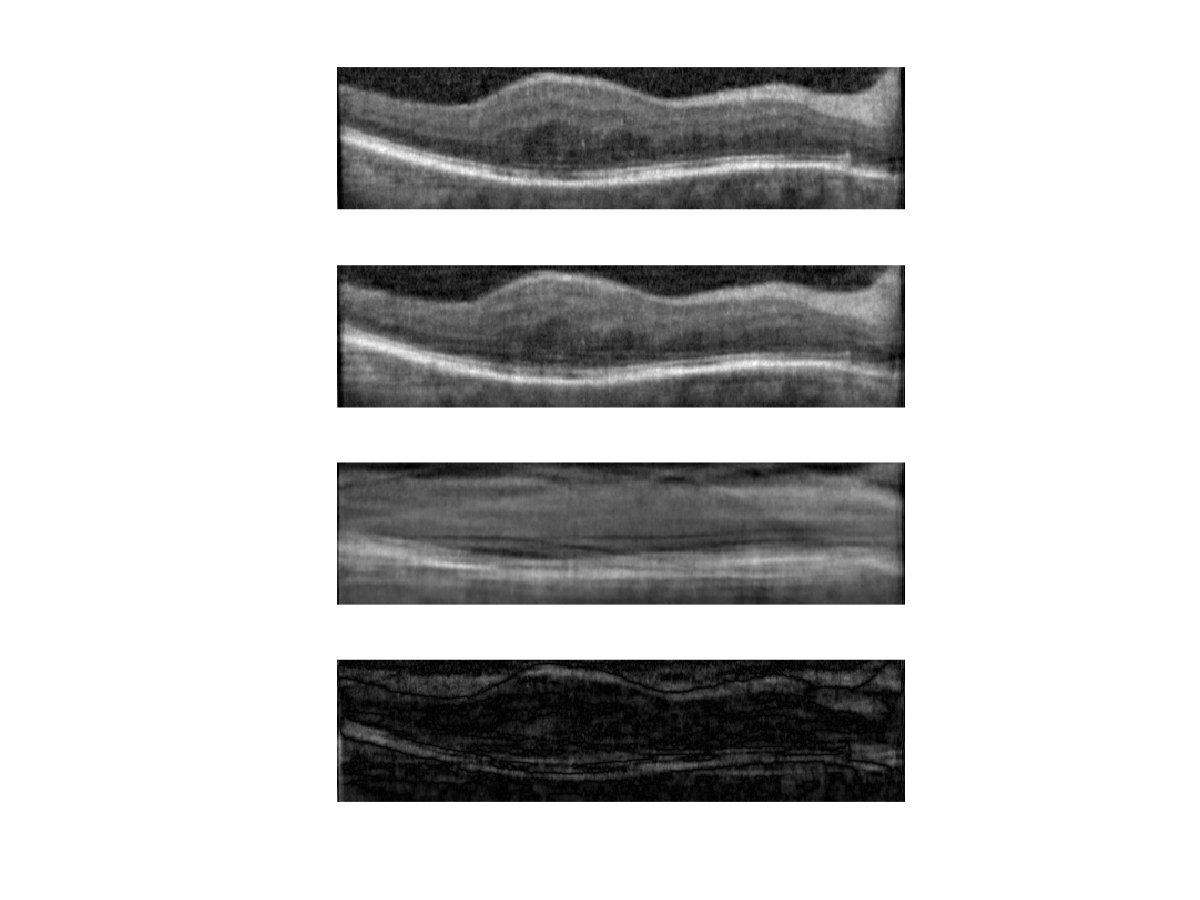
\includegraphics[width=\textwidth]{fail}
      \caption{典型失败例子}
      \label{fig:fail}
    \end{figure}


    尽管工作还存在改进的地方,但是,它为只有类别标注的中等规模的眼底黄斑区OCT成像预测病态位置信息问题,提供了一种简洁的设计思路,被证明是一种较有效的方法。



% \include{data/chap01}
% \chapter{中华人民共和国}
\label{cha:china}

\section{其它例子}
\label{sec:other}

在第~\ref{cha:intro} 章中我们学习了贝叶斯公式~(\ref{equ:chap1:bayes}),这里我们复
习一下:
\begin{equation}
\label{equ:chap2:bayes}
p(y|\mathbf{x}) = \frac{p(\mathbf{x},y)}{p(\mathbf{x})}=
\frac{p(\mathbf{x}|y)p(y)}{p(\mathbf{x})}
\end{equation}

\subsection{绘图}
\label{sec:draw}

本模板不再预先装载任何绘图包(如 \pkg{pstricks,pgf} 等),完全由用户来决定。
个人觉得 \pkg{pgf} 不错,不依赖于 Postscript。此外还有很多针对 \LaTeX{} 的
 GUI 作图工具,如 XFig(jFig), WinFig, Tpx, Ipe, Dia, Inkscape, LaTeXPiX,
jPicEdt, jaxdraw 等等。

\subsection{插图}
\label{sec:graphs}

强烈推荐《\LaTeXe\ 插图指南》!关于子图形的使用细节请参看 \pkg{subcaption} 宏包的说明文档。

\subsubsection{一个图形}
\label{sec:onefig}
一般图形都是处在浮动环境中。之所以称为浮动是指最终排版效果图形的位置不一定与源文
件中的位置对应\footnote{This is not a bug, but a feature of \LaTeX!},这也是刚使
用 \LaTeX{} 同学可能遇到的问题。如果要强制固定浮动图形的位置,请使用 \pkg{float} 宏包,
它提供了 \texttt{[H]} 参数,比如图~\ref{fig:xfig1}。
\begin{figure}[H] % use float package if you want it here
  \centering
  \includegraphics{thu-whole-logo}
  \caption{利用 Xfig 制图}
  \label{fig:xfig1}
\end{figure}

大学之道,在明明德,在亲民,在止于至善。知止而后有定;定而后能静;静而后能安;安
而后能虑;虑而后能得。物有本末,事有终始。知所先后,则近道矣。古之欲明明德于天
下者,先治其国;欲治其国者,先齐其家;欲齐其家者,先修其身;欲修其身者,先正其心;
欲正其心者,先诚其意;欲诚其意者,先致其知;致知在格物。物格而后知至;知至而后
意诚;意诚而后心正;心正而后身 修;身修而后家齐;家齐而后国治;国治而后天下
平。自天子以至于庶人,壹是皆以修身为本。其本乱而未治者 否矣。其所厚者薄,而其所
薄者厚,未之有也!

\hfill —— 《大学》


\subsubsection{多个图形}
\label{sec:multifig}

如果多个图形相互独立,并不共用一个图形计数器,那么
用 \texttt{minipage} 或者\texttt{parbox} 就可以。否则,请参看
图~\ref{fig:big1-subcaptionbox},它包含两个小图,分别是图~\ref{fig:subfig1}和
图~\ref{fig:subfig2}。推荐使用\cs{subcaptionbox},因为可以像
图~\ref{fig:big1-subcaptionbox} 那样对齐子图的标题,也可以使
用\pkg{subcaption}宏包的\cs{subcaption}(放在 minipage中,用法同\cs{caption})
或是 \pkg{subfigure} 、 \pkg{subtable}环境,像图~\ref{fig:big1-subfigure},
不要再用 \cs{subfloat}、\cs{subfigure} 和 \cs{subtable}。

\begin{figure}[h]
  \centering%
  \subcaptionbox{第一个小图形\label{fig:subfig1}}[3cm] %标题的长度,超过则会换行,如下一个小图。
    {\includegraphics[height=3cm]{thu-fig-logo}} %
  \hspace{4em}%
  \subcaptionbox{第二个小图形,注意这个图略矮些。如果标题很长的话,它会自动换行\label{fig:subfig2}}
      {\includegraphics[height=2cm]{thu-text-logo}}
  \caption{包含子图形的大图形(subcaptionbox示例)}
  \label{fig:big1-subcaptionbox}
\end{figure}


\begin{figure}[h]
  \centering%
  \begin{subfigure}{3cm}
    \includegraphics[height=3cm]{thu-fig-logo}
    \caption{第一个小图形}
  \end{subfigure}%
  \hspace{4em}%
  \begin{subfigure}{0.5\textwidth}
    \includegraphics[height=2cm]{thu-text-logo}
    \caption{第二个小图形,注意这个图略矮些。subfigure中同一行的子图在顶端对齐。}
  \end{subfigure}
  \caption{包含子图形的大图形(subfigure示例)}
  \label{fig:big1-subfigure}
\end{figure}

古之学者必有师。师者,所以传道受业解惑也。人非生而知之者,孰能无惑?惑而不从师,
其为惑也,终不解矣。生乎吾前,其闻道也固先乎吾,吾从而师之;生乎吾後,其闻道也亦
先乎吾,吾从而师之。吾师道也,夫庸知其年之先後生於吾乎!是故无贵无贱无长无少,道
之所存,师之所存也。

嗟乎!师道之不传也久矣,欲人之无惑也难矣。古之圣人,其出人也远矣,犹且从师而问焉;
今之众人,其下圣人也亦远矣,而耻学於师。是故圣益圣,愚益愚。圣人之所以为圣,愚
人之所以为愚,其皆出於此乎?爱其子,择师而教之,於其身也,则耻师焉,惑焉。彼童子
之师,授之书而习其句读者,非吾所谓传其道、解其惑者也。句读之不知,惑之不解,或师
焉,或不焉,小学而大遗,吾未见其明也。巫医、乐师、百工之人不耻相师,  士大夫之族
曰“师”曰“弟子”之云者,则群聚而笑之。问之,则曰:彼与彼年相若也,道相似也,位
卑则足羞,官盛则近谀。呜呼!师道之不复,可知矣。巫医、乐师、百工之人。吾子不齿,
今其智乃反不能及,其可怪也欤!圣人无常师。孔子师郯子、苌子、师襄、老聃。郯子之徒,
其贤不及孔子。孔子曰:“三人行,必有我师。”是故弟子不必不如师,师不必贤於弟子。
闻道有先後,术业有专攻,如是而已。

如果要把编号的两个图形并排,那么小页就非常有用了:
\begin{figure}
\begin{minipage}{0.48\textwidth}
  \centering
  \includegraphics[height=2cm]{thu-whole-logo}
  \caption{并排第一个图}
  \label{fig:parallel1}
\end{minipage}\hfill
\begin{minipage}{0.48\textwidth}
  \centering
  \includegraphics[height=2cm]{thu-whole-logo}
  \caption{并排第二个图}
  \label{fig:parallel2}
\end{minipage}
\end{figure}

李氏子蟠,年十七,好古文、六艺,经传皆通习之,不拘於时,学於余。余嘉其能行古
道,作师说以贻之。

\hfill —— 韩愈(唐)



%%% 其它部分
\backmatter

%% 本科生要这几个索引,研究生不要。选择性留下。
% 插图索引
\listoffigures
% 表格索引
\listoftables
% 公式索引
\listofequations


%% 参考文献
% 注意:至少需要引用一篇参考文献,否则下面两行可能引起编译错误。
% 如果不需要参考文献,请将下面两行删除或注释掉。
\bibliographystyle{thuthesis}
\bibliography{ref/refs}


%% 致谢
% 如果使用声明扫描页,将可选参数指定为扫描后的 PDF 文件名,例如:
% \begin{acknowledgement}[scan-statement.pdf]
\begin{acknowledgement}
  衷心感谢导师 孙延奎 教授对本人的精心指导。他们的言传身教将使
  我终生受益。

  感谢实验室全体老师和同学们的热情帮助和支
  持!本课题承蒙国家自然科学基金资助,特此致谢。

  
  \end{acknowledgement}


%% 附录

\begin{appendix}
% \includepdf[]
% \includepdf[pages=-]{trans.pdf}
% \chapter{外文资料原文}
% \includepdf[pages=-]{../ref/batch-omp.pdf}
% \chapter{翻译}
% \includepdf[pages=-, height=/textheight]{../ref/trans.pdf}
\includepdf[pages=1,pagecommand={\chapter{外文翻译} \thispagestyle{empty}}, fitpaper=true]{../ref/trans.pdf}
\includepdf[pages=2-,pagecommand={\thispagestyle{empty}}, fitpaper=true]{../ref/trans.pdf}


\end{appendix}

%% 个人简历
\begin{resume}

  \resumeitem{个人简历}

  1995 年 9 月 12 日出生于 北京市。

  2013 年 8 月考入 清华 大学 计算机科学与技术 系 计算机科学与技术 专业,攻读工学硕士学位至今。

  % 2017 年 7 月本科毕业并获得 xx 学士学位。
  % xxxx 年 9 月免试进入 xx 大学 xx 系攻读 xx 学位至今。

  \researchitem{发表的学术论文} % 发表的和录用的合在一起

  % 1. 已经刊载的学术论文(本人是第一作者,或者导师为第一作者本人是第二作者)
  \begin{publications}
    \item Yang Y, Ren T L, Zhang L T, et al. Miniature microphone with silicon-
      based ferroelectric thin films. Integrated Ferroelectrics, 2003,
      52:229-235. (SCI 收录, 检索号:758FZ.)
    \item 杨轶, 张宁欣, 任天令, 等. 硅基铁电微声学器件中薄膜残余应力的研究. 中国机
      械工程, 2005, 16(14):1289-1291. (EI 收录, 检索号:0534931 2907.)
    \item 杨轶, 张宁欣, 任天令, 等. 集成铁电器件中的关键工艺研究. 仪器仪表学报,
      2003, 24(S4):192-193. (EI 源刊.)
  \end{publications}

  % 2. 尚未刊载,但已经接到正式录用函的学术论文(本人为第一作者,或者
  %    导师为第一作者本人是第二作者)。
  \begin{publications}[before=\publicationskip,after=\publicationskip]
    \item Yang Y, Ren T L, Zhu Y P, et al. PMUTs for handwriting recognition. In
      press. (已被 Integrated Ferroelectrics 录用. SCI 源刊.)
  \end{publications}

  % 3. 其他学术论文。可列出除上述两种情况以外的其他学术论文,但必须是
  %    已经刊载或者收到正式录用函的论文。
  \begin{publications}
    \item Wu X M, Yang Y, Cai J, et al. Measurements of ferroelectric MEMS
      microphones. Integrated Ferroelectrics, 2005, 69:417-429. (SCI 收录, 检索号
      :896KM)
    \item 贾泽, 杨轶, 陈兢, 等. 用于压电和电容微麦克风的体硅腐蚀相关研究. 压电与声
      光, 2006, 28(1):117-119. (EI 收录, 检索号:06129773469)
    \item 伍晓明, 杨轶, 张宁欣, 等. 基于MEMS技术的集成铁电硅微麦克风. 中国集成电路,
      2003, 53:59-61.
  \end{publications}

  \researchitem{研究成果} % 有就写,没有就删除
  \begin{achievements}
    \item 任天令, 杨轶, 朱一平, 等. 硅基铁电微声学传感器畴极化区域控制和电极连接的
      方法: 中国, CN1602118A. (中国专利公开号)
    \item Ren T L, Yang Y, Zhu Y P, et al. Piezoelectric micro acoustic sensor
      based on ferroelectric materials: USA, No.11/215, 102. (美国发明专利申请号)
  \end{achievements}

\end{resume}


%% 本科生进行格式审查是需要下面这个表格,答辩可能不需要。选择性留下。
% 综合论文训练记录表
% \includepdf[pages=-]{scan-record.pdf}
\end{document}
